\section{Experiments} 

We have implemented our method in python\footnote{The entirety of the code,
    networks, datasets, and properties utilized in our evaluation will be made
    available via a publicly hosted code repository in the
camera ready version.}., utilising the NumPy
%\cite{numpy}
library for linear algebra operations and the SciPy
%\cite{scipy}
library for an
implementation of \hcluster.
We have used a linkage-matrix \cite{scipy-hcluster-linkage}  based
data structure to store the tree, and have precomputed and cached several
operations that may need to be repeated every refinement iteration. This allows
us to quickly perform the merge and split operations and calculate the
scores (Section \ref{s:refinement}), without having to do (relatively)
expensive tree traversal operations in each iteration of the abstraction
refinement loop. 

Using this implementation, we have performed three sets of experiments to
demonstrate the usefulness of our technique. In several safety critical
settings, such as medical diagnosis and collision detection, where \dnn are
deployed as classifiers, false negative classification with respect to some
classes are highly undesirable. In the first set of experiments, we show that
our abstraction technique can be leverage to obtain effective compression of
\dnn in such settings with a guarantee that the compression does not introduce
any new false negative classifications (Section \ref{s:exp-mnist-comp}). In our
second set of experiments, we demonstrate how our technique may be used to
obtain abstract networks with the aim of proving a given property, plotting the
number of spurious counterexamples introduced as the size of the abstract
network reduces (Section \ref{s:exp-mnist-rob}). Finally, in the last set of
experiments, we show how our technique may be used in a CEGAR loop
\cite{cegar-nn} to verify the \acasxu properties. We utilized \abcrown as the 
solver in the backend for these experiments. 

If the \abs produced has multiple neurons with the exact same set of incoming
edges in the same layer, these neurons compute the same function and are
redundant. Therefore, as an added optimization step, we safely \textit{re-merge}
them by taking the sum of the outgoing edges. Note that this does not change the
behavior of \abs.

The experimental results in Tables
\ref{t:mnist-compr-summary}, 
\ref{t:acas-ncex} , \ref{t:acas-verif} and Figures \ref{f:acas-ncex-samples},
\ref{f:acas-ncex-pgd}, \ref{f:acas-verif-ref},
\ref{f:mnist-class} were
run on a machine running on an Intel(R) Core(TM) i7-9700K with 8 CPUs running at
3.60GHz, having 16 GB RAM and running Ubuntu 22.04 LTS. The results in
Figures \ref{f:mnist-prop-samples}, Figures \ref{f:mnist-prop-pgd} and Table
\ref{t:mnist-prop-summary} were produced on a 
machine running on an Intel(R) Core(TM) i7-13700 with 24 CPUs running at
5.20GHz, having 32 GB RAM and running Ubuntu 23.10.

\subsection{Compression with Guarantees on Critical Classes}
\label{s:exp-mnist-comp}

In several safety-critical applications of \dnn as classifiers, there are
certain `critical` classes for which a false negative classification is far more
dangerous than a false positive one. For example, for medical diagnosis and
collision detection, a false negative is far more dangerous than a false
positive.

Safety critical analysis of neural networks is highly sensitive to the size of
the network. While several neural network compression techniques exist 
\cite{dnn-compression}, they do not provide formal guarantees 
connecting the behavior of the compressed network and the original network.
Similarly, although existing semantic abstraction techniques have been proposed
as a way to compress neural networks, the guarantees provided by such 
techniques are of an empirical nature \cite{lin-comb-abs-jan}.
This lack of guarantees also limits the usefulness of these compression
techniques as optimisation steps when deploying a network to a
resource-constrained environment. 

Our theoretical framework for abstraction allows us to produce compressed
networks with the formal guarantee that the abstraction process will not
introduce any new false negatives. We do this by marking the output neuron $n_c$
corresponding to the critical class in the output layer as \inc, and all other
neurons in that layer as \dec.  Then, for any input that \cnc classified into
the critical class, $n_c$ will have the largest value in the
output layer, and as it has been marked as \inc, it will continue to have the
largest value in the output layer for \abs as well. Thus, the
abstract network will also classify this input as critical. We will however pay
for this compression by introducing false positives.

We demonstrate the effectiveness of our abstraction method as a
compression-with-guarantees technique via some experiments on \mnist. We set the
class '0'
as the critical class. Then, starting with the fully merged network, we
iteratively perform refinements while measuring the accuracy, false/true
positive/negative rates. We perform this experiments with four strategies of
selecting the culprit neuron $\gamma$ to refine:

\begin{itemize}
    \item \textit{random}: Choose $\gamma$ at random. This serves as a
        baseline.
    \item \textit{samples}: An uniform sampling of the input space is used to
        generate a large set of \gencex $\vct{\beta}$. These are used to
        calculate the score and select $\gamma$ as in 
        \ref{s:refinement}.
    \item \textit{pgd}: The $\vct{\beta}$ are generated via a PGD
        \cite{pgd, pgd-attack} attack on \abs, and then used in a manner similar
        to \textit{samples}.
    \item \textit{samples-pgd}: Initial refinement steps are done following the
        \textit{samples} strategy, switching to \textit{pgd} when all the
        samples have been exhausted.
\end{itemize}

We use the \abcrown implementation for \pgd.

\begin{figure}
    \begin{subfigure}{0.475\linewidth}
        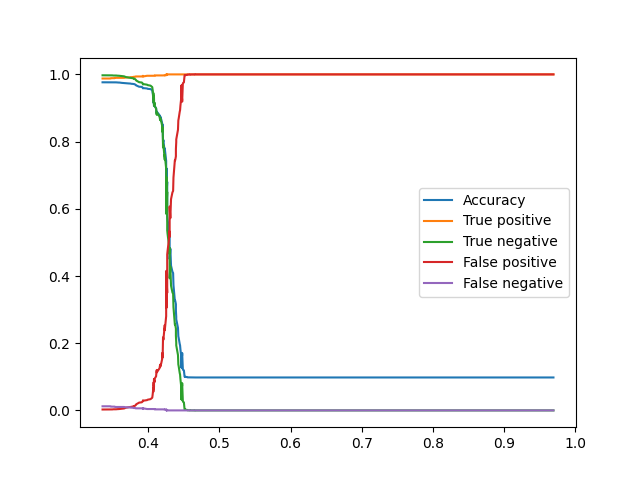
\includegraphics[scale=0.275]{figs/mnist-compr-4-256-samples.png}
        \caption{}
        \label{f:mnist-compr-samples}
    \end{subfigure}
    \begin{subfigure}{0.475\linewidth}
        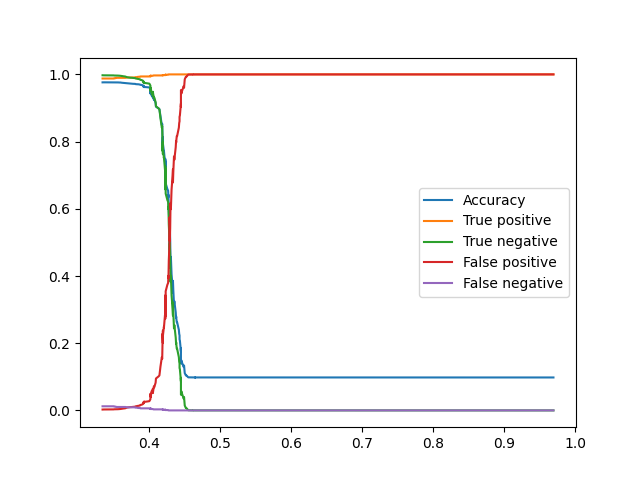
\includegraphics[scale=0.275]{figs/mnist-compr-4-256-pgd-after-samples.png}
        \caption{}
        \label{f:mnist-compr-samples-pgd}
    \end{subfigure}
    \caption{Accuracy and True/False Positive/Negative Rates vs Reduction Rate
        plot for \mnist of size $4 \times 256$ with critical class 0. Refinement
    done via the \textit{samples-pgd} and \textit{samples} method in
    \ref{f:mnist-compr-samples} and \ref{f:mnist-compr-samples-pgd} 
    respectively. }
    \label{f:mnist-class}
\end{figure}

Figure \ref{f:mnist-class} shows some typical plots of the true/false
negative/positive rates (y-axis) against reduction rate (x-axis). Note that the
reduction rate plotted is with respect to the size of the network obtained after
\inc-\dec splitting. While this may mean that \abs produced may be greater in
size than the original network, note that in such an \abs each neuron can be
cleanly classified as \inc or \dec with respect to a property of interest, which
may make formal analysis simpler. Indeed, it has been seen that such \abs, while
larger, may be easier to verify \cite{cegar-nn}.

We notice that, as guaranteed by the theory, the false negative rate never
increases, even as the reduction rate approaches close to $100\%$. In fact, the
false negative rate improves, as some of the points that are going
to be newly classified as positive may in fact be true positives.  
However, as discussed before, we do pay for the compression by introducing false
positives, which we see in the graph. 

We also find in the graph that there is a
small window of reduction rate values where almost all of the improvement in the
false positive rate occurs. This indicates that we eventually are able make 
significant improvements in false positive rate while sacrificing reduction rate
as little as possible. Thus our technique is able to use the semantic
information to order and undo merge operations in an optimal way.

\begin{table}
\begin{tabular}{|c|c|c|c|c|}
\hline
Net Size     & Refinement  & Reduction & False Positives & Steps  \\ 
\hline
$2\times256$ & random      & 50.0 \%   & 0.2  \%         &  923   \\  
$4\times256$ & random      & 50.0 \%   & 0.2  \%         & 1917    \\ 
$6\times256$ & random      & 50.0 \%   & 0.2  \%         & 2999    \\ 
$2\times256$ & samples     & 45.7 \%   & 0.3  \%         &  326    \\ 
$4\times256$ & samples     & 38.7 \%   & 2.2  \%         & 1037    \\ 
$6\times256$ & samples     & 45.5 \%   & 0.2  \%         & 2425    \\ 
$2\times256$ & pgd         & 53.4 \%   & 95.6 \%         &   85    \\ 
$4\times256$ & pgd         & 96.9 \%   & 100  \%         &    0    \\ 
$6\times256$ & pgd         & 30.6 \%   & 94.1 \%         & 1482    \\ 
$2\times256$ & samples-pgd & 46.0 \%   & 0.5  \%         &  316    \\ 
$4\times256$ & samples-pgd & 39.2 \%   & 2.1  \%         & 1027    \\ 
$6\times256$ & samples-pgd & 45.5 \%   & 0.2  \%         & 2425    \\ 
\hline
\end{tabular}
\caption{Summary of \mnist compression Results}
\label{t:mnist-compr-summary}
\end{table}

Table \ref{t:mnist-compr-summary} summarises the results from running all the
\mnist compression experiments. For each instance, we report the best reduction
rate achieved for a network whose false positive rate was close to the best
false positive rate seen
throughout the refinement process. Note that we currently do not stop our
refinement loop at the precise point where this network is produced, but may
continue to refine beyond this point.

Firstly, we find that \textit{pgd} performs relatively poorly, with fewer
refinements being performed, producing an small network that is too abstract and
has a high false positive rate. This is because the \abcrown
implementation of \pgd fails to find a spurious counterexample early on in the
refinement process for these instances, leading to early termination. 

The other instances and methods seem to perform
comparably on the same network in terms of reduction rate and false positive
rate. This is evidence for the fact that, regardless of what specific strategy
is used to find $\gamma$ in the refinement process, our framework uses the
semantic information to guide the refinement to reach equally optimal \abs.

Further, we see some difference in the number of steps taken by \textit{random}
and the other methods in finding the abstract network. This indicates that while
the \abs reached may be equally optimal, 
heuristics for finding $\gamma$ indeed
shortens the search for the refined network.

We note that in \cite{cleverest-nn}, an eager PGD-attack before each solver call
has been effectively used to accelerate the CEGAR loop. We do not see such
benefits from using PGD, and instead observe that the global view given by
the large number of samples in the \textit{samples} method performs better.
While the relative performance of \textit{pgd} and \textit{samples} may be
different for a different set of target network and property, our framework
allows the use of either, and in-fact, any other method for generating the
counterexamples.

\subsection{Eliminating Spurious Counterexamples}
\label{s:exp-mnist-rob}

In this section, we explore how well our abstraction refinement process is able
to remove spurious counterexamples. We start with the abstract network and
iteratively perform refinements, measuring the number of spurious
counterexamples at each step. 

\begin{figure}

    \begin{subfigure}{0.475\linewidth}
        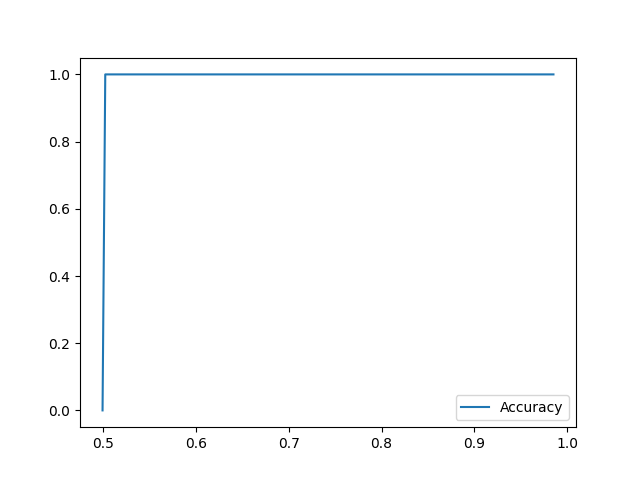
\includegraphics[scale=0.275]{figs/mnist_2_256_prop_0_0.03_samples.png}
        \caption{}
        \label{f:mnist-prop-samples}
    \end{subfigure}
    \begin{subfigure}{0.475\linewidth}
        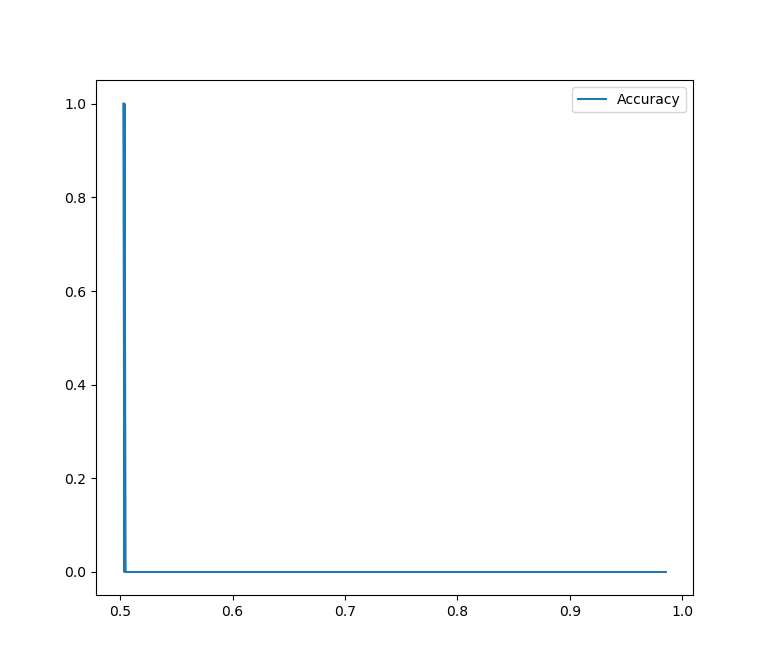
\includegraphics[scale=0.275]{figs/mnist_2_256_prop_0_0.03_pgd.png}
        \caption{}
        \label{f:mnist-prop-pgd}
    \end{subfigure}

    \begin{subfigure}{0.475\linewidth}
        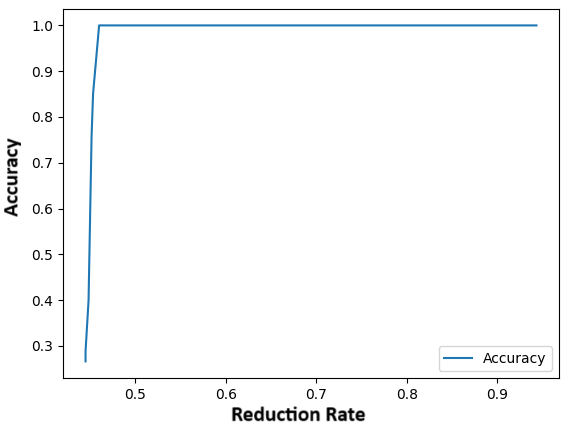
\includegraphics[scale=0.275]{figs/acas_ncex_5_8_3_samples.png}
        \caption{}
        \label{f:acas-ncex-samples}
    \end{subfigure}
    \begin{subfigure}{0.475\linewidth}
        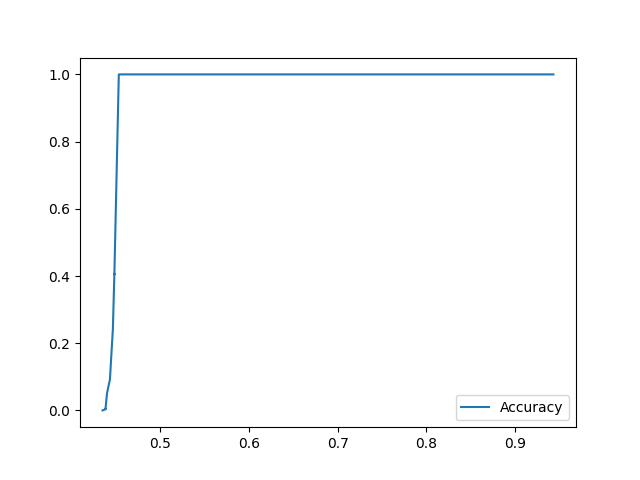
\includegraphics[scale=0.275]{figs/acas_ncex_5_8_3_pgd.png}
        \caption{}
        \label{f:acas-ncex-pgd}
    \end{subfigure}

    \caption{
        Spurious counterexample vs Reduction Rate plot for \mnist of size $2
        \times 256$ with $\epsilon$-Robustness property are given in 
        \ref{f:mnist-prop-samples} and \ref{f:mnist-prop-pgd}. 
        Spurious counterexample vs Reduction Rate plot for \acasxu network 5-8,
        property 3 in \ref{f:acas-ncex-samples} and \ref{f:acas-ncex-pgd}
        Refinement done via the \textit{pgd} method in
        \ref{f:mnist-prop-pgd} and \ref{f:acas-ncex-pgd} and 
        via \textit{samples} method in \ref{f:mnist-prop-samples} and
        \ref{f:acas-ncex-samples}.
    }
    \label{f:ncex}
\end{figure}

We experimented with two sets of networks and properties: \mnist with
adversarial robustness properties and \acasxu with the properties from
\cite{reluplex}. For each, we tried the 4 strategies for choosing $\gamma$ from
Section \ref{s:exp-mnist-comp}.
Figure \ref{f:ncex} shows some typical plots
for these experiments. Here the x-axis measures the reduction rate with respect
to the \inc-\dec split networks and the y-axis is the rate of true
counterexamples within a random sample - thus a low value indicates a good
abstraction.

Similar to Section \ref{s:exp-mnist-comp}, we see that there is a small window
of reduction rate values where most of the improvement in over-approximation
occurs. As before, we believe that this is evidence that we are able to use
semantic information and undo merge operations optimally.

\begin{table}
\begin{tabular}{|c|c|c|c|c|}
    \hline
    Net Size     & Refinement  & Reduction & Cex. Rate & No. Steps \\
    \hline
    $2\times256$ & random      & $49.1\%$  & $  0\%$  & $ 899$    \\
    $4\times256$ & random      & $49.6\%$  & $  0\%$  & $1929$    \\
    $6\times256$ & random      & $49.7\%$  & $  0\%$  & $2818$    \\
    $2\times256$ & samples     & $50.3\%$  & $  0\%$  & $  27$    \\
    $4\times256$ & samples     & $49.9\%$  & $  0\%$  & $ 648$    \\
    $6\times256$ & samples     & $47.9\%$  & $  0\%$  & $1199$    \\
    $2\times256$ & pgd         & $50.4\%$  & $  0\%$  & $  28$    \\
    $4\times256$ & pgd         & $49.8\%$  & $  0\%$  & $ 648$    \\
    $6\times256$ & pgd         & $47.9\%$  & $  0\%$  & $1203$    \\
    $2\times256$ & samples-pgd & $50.4\%$  & $  0\%$  & $  28$    \\
    $4\times256$ & samples-pgd & $49.8\%$  & $  0\%$  & $ 648$    \\
    $6\times256$ & samples-pgd & $47.9\%$  & $  0\%$  & $1201$    \\
    \hline
\end{tabular}
\caption{Summary of \mnist Results on a single robustness property }
\label{t:mnist-prop-summary}
\end{table}

Table \ref{t:mnist-prop-summary} summarizes our observations for \mnist. We
choose a network to report the reduction rate in a manner similar to Section
\ref{s:exp-mnist-comp} and make similar observations. However, for these benchamrks 
PGD-attack also had a similar reduction rate and was able to eliminate the
counterexamples. Infact all the methods arrive at
\abs with similar reduction and counterexample rates and are able to eliminate all
counterexamples. Again, we see that \textit{random} takes more number of steps
to arrive at the \abs, indicating that heuristics for finding $\gamma$ shortens
the search for \abs.

\begin{table}
\begin{tabular}{|c|c|c|c|c|}
\hline
Benchmark   & Reduction  & \% Sp. Cex. & Steps    \\
\hline
samples     & 45.5\%     &  13.0\%     & 294.111  \\
random      & 50.9\%     &  3.6\%      & 512.011  \\
pgd         & 50.8\%     &  16.1\%     & 235.606  \\
samples-pgd & 45.1\%     &  5.3\%      & 299.272  \\
\hline
\end{tabular}
\caption{Summary of \acasxu, measuring the percentage of spurious counterexample }
\label{t:acas-ncex}
\end{table}

Table \ref{t:acas-ncex} summarises the results for the \acasxu networks. Here,
we see that all 4 strategies for selecting $\gamma$ seem to produce much more
similar \abs. Indeed, PGD-attack was much more successful in finding
$\vct{\beta}$ for these networks, only producing slightly more counterexamples.
Again, we find that \textit{random} takes many more steps but arrives at a
network of similar size.

\subsection{Verification of \acasxu}

In these set of experiments, we have taken the \acasxu set of
networks and properties and attempt to verify them using a \cegar approach. We
use our technique to generate the abstraction, and attempt to verify the
property on the abstract network using an existing neural network verification
solver. If the solver returns a counterexample, and if that counterexample is
not spurious, we use that counterexample as a reference point for score
calculation  to select the culprit neuron (\ref{s:refinement}). With the culprit
neuron selected, we then refine the network.

\begin{table}
%\footnotesize
\begin{tabular}{ |c|c|c|c| }
\hline
Benchmark   & \% Verified & Size     & Time \\ 
\hline
prop-Safe   &   64\%      & 339      & 11.1  \\
prop-Unsafe &   93\%      & 140      & 10.0  \\
adv-unsafe  &  100\%      & 18       & 1.2   \\
\hline                                                                
\end{tabular}
\caption{Summary of \acasxu verification. `prop-Safe/Unsafe' refers to
safe/unsafe instances of the original properties from \cite{reluplex},
`adv-unsafe' refers to adversarial properties from \cite{cegar-nn}. }
\label{t:acas-verif}
\end{table}

The results are summarised in table \ref{t:acas-verif}. The solver we used was
\abcrown. The average times reported here do not include instances where the
verification failed due to timeout.

We notice that for the unsafe cases, we are able to refute the
properties via a counterexample obtained on a significantly smaller network. In
fact, for most networks, we are able to refute based on a counterexample from
the fully abstracted network of size $18$. Note that since we use only two classes in our
fully abstracted network as opposed to 4 in \cite{cegar-nn}, the size of this
network is significantly smaller. 

For safe cases, we see only negligible improvement in the size of the network.
We believe that this is because for these benchmarks, there is not much room for
improvement via abstraction. We are also able to only verify a smaller
percentage of these benchmarks, because the underlying solver call would time
out on mid-sized abstract networks, stalling
the CEGAR loop. We note that some timeouts were also reported in
\cite{cegar-nn}, and thus may be expected.

\begin{figure}
    \begin{subfigure}{0.475\linewidth}
        \centering
        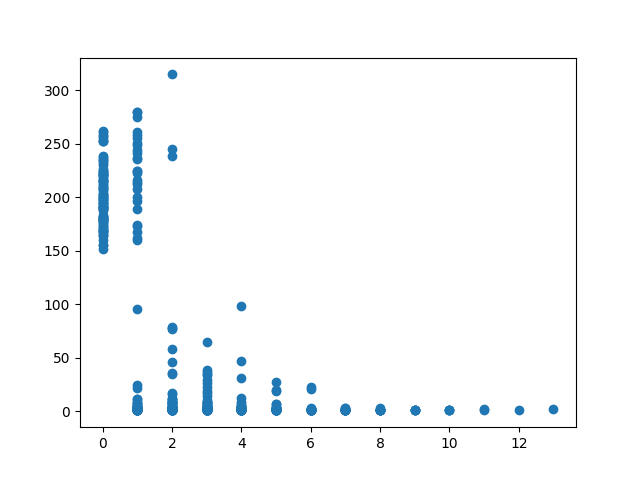
\includegraphics[scale=0.25]{figs/acas_verif_ref_sizes_safe.png}
        \caption{}
        \label{f:acas-verif-ref-safe}
    \end{subfigure}
    \begin{subfigure}{0.475\linewidth}
        \centering
        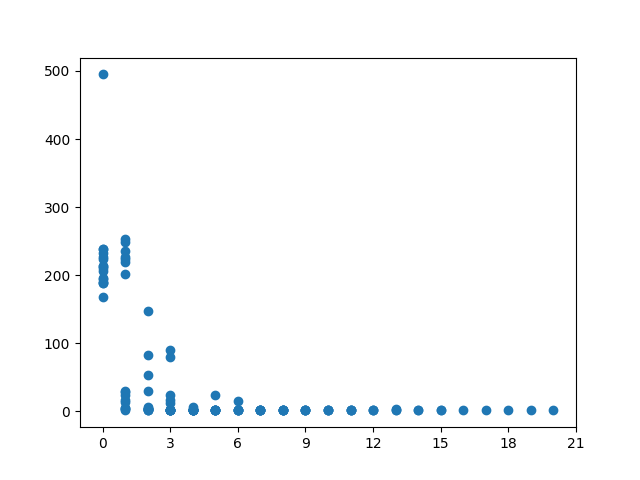
\includegraphics[scale=0.25]{figs/acas_verif_ref_sizes_unsafe.png}
        \caption{}
        \label{f:acas-verif-ref-unsafe}
    \end{subfigure}
    \caption{Number of neurons un-merged vs solver call number for \acasxu. Safe
        cases in \ref{f:acas-verif-ref-safe}, unsafe in
        \ref{f:acas-verif-ref-unsafe}}
    \label{f:acas-verif-ref}
\end{figure}

In Figure \ref{f:acas-verif-ref} we show scatter plots of the number of neurons
un-merged in between each solver call. We observe that the number is highly
dependent on the specific benchmark instance,
and on how late in the \cegar loop we are. This is unlike previous methods
that arbitrarily and uniformly choose the number of un-merges
\cite{cegar-nn} to be performed between each solver call. We believe
that this is more evidence for the fact that our framework is able to take into
account the larger semantic context of each refinement step. 

In our experiments we also find that the time taken for a solver call are more
dependent on the particular solver, solver configuration and benchmark than on
the size of the network. Thus it may seem that the effort needed to verify a
network is dependent on other factors than simply the size of the network. While
this may be interesting to explore in future work, we nonetheless argue that
network size is a relevant metric. This is as more and more solvers are designed
and optimized for various kinds of networks, the underlying worst case
performance will almost certainly remain exponential in the size of the network
\cite{reluplex}.

